\chapter{System Identification Fundamentals}\label{Lab:1}
Low-pass filters are ubiquitous. They can be found in the hardware of
audio processing chips, or the software of image editing tools. As you may
recall from a course on Signals and Systems theory\footnote{If you haven't
taken a course in Signals and Systems, speak to your Lab Instructor on
knowledge you may be lacking.}, a low-pass filter
is a system that, generally speaking, rejects high-frequency signals while
``passing through'' low-frequency signals. In this lab you will be asked
to analyze a low-pass filter block and determine its parameters via a time
domain approach. This is not meant to be a difficult lab and is instead
designed to give you a sense of the lab format. However, it will put to the
test your knowledge of signals and systems. If you have forgotten your
Laplace transforms, this is a good time to remind yourself of them!

In the real world, our models are rarely perfect. The techniques
you learn here generalize nonetheless. Whenever you confront a novel system,
devise a generic model that you think characterizes its behaviour and then
come up with experiments that expose its characteristics; this gives you
estimates of the generic model's parameters that best fit the actual system.
We will encounter such a situation in a future lab.

\section{Objectives}
The primary objectives of this lab are to
\begin{enumerate}[label=(\arabic*)]
  \item{
    \textbf{Install} MATLAB, Simulink and required toolboxes.
    Alternatively, \textbf{connect remotely} to
    \url{engterm.uwaterloo.ca} or any other lab computer of your choice
    that has MATLAB.
  }
  \item{
    Understand how to \textbf{open} and \textbf{modify}
    a Simulink diagram and how to run a simulation.
  }
  \item{
    Understand how to \textbf{log} signals for future inspection.
  }
  \item{
    Understand how to \textbf{plot} figures and capture them.
  }
  \item{
    Understand the theory behind first-order low-pass systems.
  }
  \item{
    Understand how to \textbf{identify} a first-order low-pass system.
  }
\end{enumerate}
This is not a particularly long lab, but you may have trouble as it is
very likely your first encounter with Simulink. As a result, I suggest you
give you and your partner time to work through the lab and the problems.
I also recommend you spend some time by yourself exploring Simulink so as to
reduce the amount of time you spend on future labs.

\section{Experimental Procedure}
This entire lab will be done using the ``\texttt{Lab\_1.slx}'' Simulink model.
In there you will
find a number of blocks already placed for you in an open loop configuration:
\begin{itemize}
  \item{a signal generator,}
  \item{a summing junction,}
  \item{an adjustable gain block,}
  \item{a ``plant'', the system we are going to analyze, and}
  \item{a terminator.}
\end{itemize}
%
The plant --- labelled \(P(s)\) in the diagram --- can be assumed to be a
transfer function taking the form
\[
  P(s) = \frac{b T}{s + a T},
\]
where \(a, b > 0\) and \(T \in \{10, 100\}.\) Your goal is to use the
techniques described in the following subsections to estimate the parameters
\(a,\) \(b\) and \(T\) for your plant. This process is known as
\textbf{system identification} and it is a critical precursor to control
design. How can we design a controller if we don't even know the parameters
of the system we wish to control?

\subsection{Acquiring the Bandwidth in Time-Domain}
The goal of this portion of the lab is to acquire the bandwidth of the
given linear system. What is the bandwidth? To understand and acquire it,
we must first know what the DC gain of a system is.
%
\begin{definition}[label={def:lab1:dcgain}]{DC Gain}
  Let \(G(s)\) be a \emph{stable} transfer function
  that maps an input signal \(U(s)\) to an
  output \(Y(s).\) The \textbf{DC gain} of \(G(s)\) is \(G(0)\) and,
  if \(u(t) = A \mathbf{1}(t)\) for \(A \in \Real,\) it satisfies the relation
  \[
    \lim_{t\to \infty} y(t) = A G(0).
  \]
\end{definition}
%
Observe that the DC gain \(G(0)\) is called precisely that because when we
apply a square (DC-like; step) signal change, the system's output converges
to the amplitude of the input times \(G(0).\)
%
Instead of computing the DC gain by evaluating the system's response to a step
input, we take a different approach.
%
\begin{procedure}[label={proc:lab1:p1}]
  You will acquire the DC gain of the plant \(P(s)\). Follow these steps:
  \begin{enumerate}[label=(\arabic*)]
    \item{
      \textbf{Open} the signal generator block, and set the
      \textbf{amplitude} to be \(1\) and the \textbf{frequency}
      to be \(\SI{0.5}{Hz}.\) This signal is so low frequency that it
      emulates a constant signal.
    }
    \item{
      \textbf{Run} the script \texttt{generate\_lab\_1\_plot.m} and inspect
      Figure 1, which depicts the input and output signal.
    }
    \item{
      \textbf{Measure the amplitudes} of the input and output signals
      respectively when the system is in steady-state. In simulation, this
      amounts to performing this measurement near the end of the simulation
      time.
    }
    \item{
      \textbf{Estimate} the DC gain by dividing the output amplitude
      by the input amplitude. \emph{Remember, we chose the input amplitude
      to be \(1\)!}
    }
  \end{enumerate}
\end{procedure}
%
\begin{figure}
  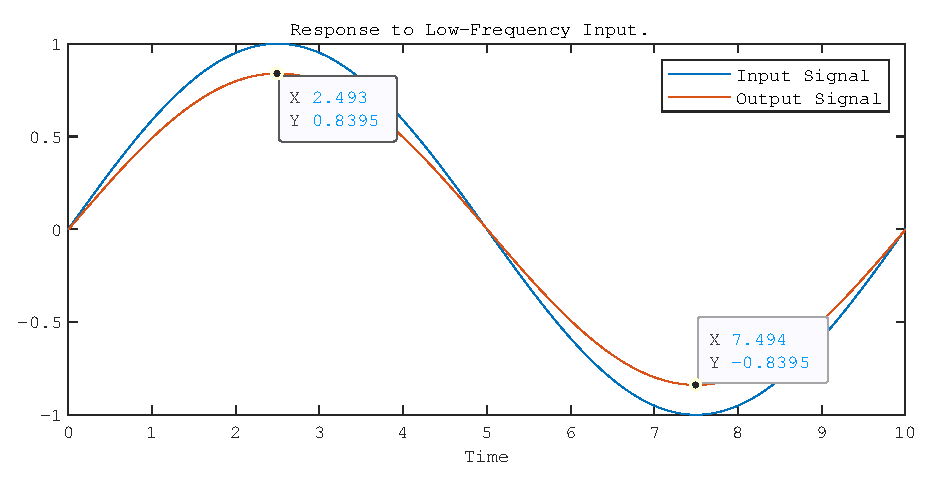
\includegraphics{images/Lab_1_LowFrequency.eps}
  \caption[Low Frequency Response of a Low-Pass Plant]{The low-frequency response to my low-pass plant \(P(s).\) The gain
  at this low frequency is \(0.8395.\) Can you see why? What is the DC
  gain approximately?}
  \label{fig:lab1:lowfreq}
\end{figure}
%
\begin{figure}
  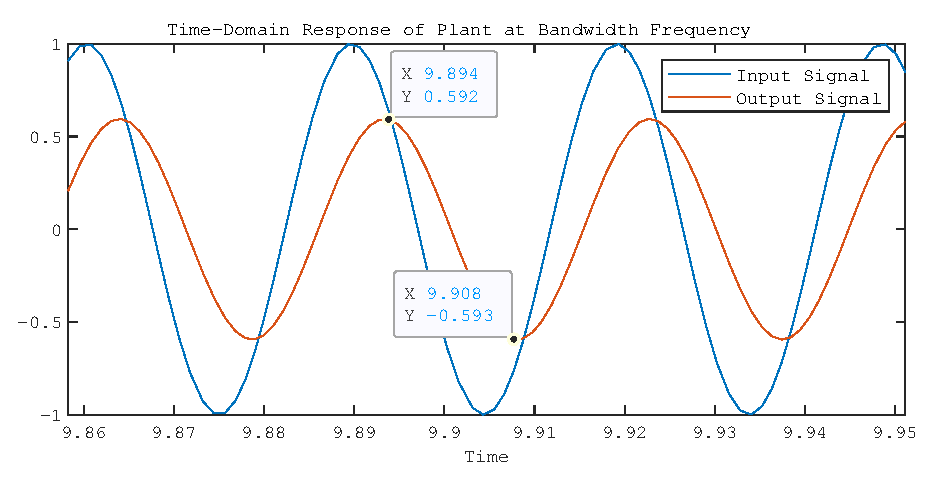
\includegraphics{images/Lab_1_Bandwidth.eps}
  \caption[Time-Domain Response of a First-Order System at the Bandwidth Frequency]{The response to my \(P(s)\) at the bandwidth frequency.
  Can you see why this is the bandwidth frequency for my plant?}
  \label{fig:lab1:bandwidth}
\end{figure}
%
\begin{deliverable}[label={lab1:d1}]
  \textbf{Record} your estimated DC gain and \textbf{capture} the generated
  figure with the cursors you used to measure the amplitudes.
  Your figure should like Figure~\ref{fig:lab1:lowfreq}.
\end{deliverable}
%
For low-pass systems, as we increase the frequency of the input, we will
observe, the output amplitude \emph{decreases}. The bandwidth frequency
is the frequency that marks the point where we distinguish between the
``low'' frequency inputs a low-pass system sustains and the ``high'' frequency
inputs a low-pass system rejects.
%
\begin{definition}[]{Bandwidth}
  Let \(G(s)\) be a proper transfer function
  that maps an input signal \(U(s)\) to an output \(Y(s).\)
%
  Say the input is a sinusoid of the form \(A \cos(\omega t)\) with amplitude
  \(A.\) In steady-state, the amplitude of \(y(t)\) converges to a constant
  \(B.\) The \textbf{gain at frequency \(\omega\)} is
  \(\left\|G(j\omega)\right\| = \frac{B}{A}.\)
%
  The \textbf{bandwidth (frequency)} of \(G(s)\) is the \emph{smallest}
  frequency \(\omega\) which satisfies
  \[
    \frac{1}{\sqrt{2}} = \frac{\left\|G(j\omega)\right\|}{\left\|G(0)\right\|}.
  \]
\end{definition}
%
What is the definition above trying to characterize? The
gain is the multiplier between the input amplitude and output amplitude. For
a low-pass system, this gain decreases as a function of input frequency. The
bandwidth frequency is the frequency where this gain has fallen, in comparison
to the DC gain, by factor of \(\sqrt{2}.\) This is further demonstrated
by the difference in response we observe between Figure~\ref{fig:lab1:lowfreq}
and Figure~\ref{fig:lab1:bandwidth}. Note how much smaller the output signal
is in the response with higher frequencies in comparison to the response
with lower frequencies.
%
\begin{procedure}[label={proc:lab1:p2}]
  You will acquire the bandwidth frequency of the plant \(P(s)\).
  Follow these steps:
  \begin{enumerate}[label=(\arabic*)]
    \item{
      \textbf{Predict} the amplitude of the steady-state output at the
      bandwidth frequency. As an example, if your DC gain is \(0.8395\) then
      the ratio between the input signal amplitude and the output signal
      at the bandwidth frequency is
      \[
        \frac{0.8395}{\sqrt{2}}.
      \]
      If my input signal has amplitude \(1,\) then I should look for
      an output signal amplitude with the above value.
    }
    \item{
      \textbf{Open} the signal generator block, and set the
      \textbf{amplitude} to be \(1\) and
      the \textbf{frequency} to be \(\SI{0.5}{Hz}.\)
      \label{lab1:p2:2}
    }
    \item{
      \textbf{Run} the script \texttt{generate\_lab\_1\_plot.m} and inspect
      Figure 1, which depicts the input and output signal.
    }
    \item{
      \textbf{Measure the amplitudes} of the output signal
      when the system is in steady-state.
      \label{lab1:p2:4}
    }
    \item{
      If the amplitude isn't what you want, repeat Steps~\ref{lab1:p2:2} through~\ref{lab1:p2:4} with a different frequency. Increase or decrease
      by orders of magnitude to speed up the process!
    }
    \item{
      If the amplitude is what you predicted, \textbf{record} the frequency
      of the input you used to achieve the result.
    }
  \end{enumerate}
\end{procedure}
%
\begin{deliverable}[label={lab1:d2}]
  At the bandwidth frequency,
  \textbf{capture a figure} of the input and output signal. It should look
  like Figure~\ref{fig:lab1:bandwidth}. Pay close attention to the time
  axis; it has been scaled to make the signal easy to measure and to visualize.
\end{deliverable}
%
Having acquired the bandwidth for the open loop system, we now investigate
the closed loop system.
%
\begin{figure}
  \centering
  \begin{tikzpicture}[x=1in, y=1in]
    \node [draw, block] (Controller) {\(K_p\)};
    \node [draw, block, right=0.5 of Controller] (Plant) {\(P(s)\)};
    \node [draw, summer, left=0.5 of Controller] (Sum) {};
    \node [below=0.5 of Sum] (BelowSum) {};

    \draw [arrow, signal]
      (Controller.east) -- (Plant.west)
      node [below left, annotate] {\(u\)};
    \draw [arrow, signal]
      (Plant.east)
      --
      +(0.35, 0)
      |-
      (BelowSum.base)
      --
      (Sum.south)
      node [below right, annotate] {\(-\)};
    \draw [arrow, signal]
      (Sum.east) -- (Controller.west);
    \draw [arrow, signal]
      ($(Sum.west)+1*(-0.5, 0)$) -- (Sum.west)
      node [below left, annotate] {\(r\)};
    \draw [arrow, signal]
      (Plant.east) -- +(0.7, 0)
      node [below, annotate] {\(y\)};
  \end{tikzpicture}
  \caption[Closed-Loop Diagram for Lab 1]{
    Closing the loop around the Plant \(P(s)\) for Lab 1.
  }
  \label{fig:lab1:closing-loop}
\end{figure}
%
\begin{procedure}[label={proc:lab1:p3}]
  Now \textbf{close the loop} around the slider gain and plant \(P(s).\) That
  is, connect your diagram so that it looks like Figure
  \ref{fig:lab1:closing-loop}. Then \textbf{set} the slider gain to
  your group provided parameter value \(Kp.\)
  Repeat Procedures~\ref{proc:lab1:p1} and~\ref{proc:lab1:p2} for the
  closed-loop system depicted in Figure~\ref{fig:lab1:closing-loop}.
\end{procedure}
%
\begin{deliverable}[label={lab1:d3}]
  Repeat Deliverables~\ref{lab1:d1} and~\ref{lab1:d2} for the closed-loop
  system discussed in Procedure~\ref{proc:lab1:p3}
\end{deliverable}

\subsection{Acquiring the Settling Time and Time Constant}
In this section of Lab 1 we take a different approach to estimating the plant
parameters. Instead of feeding in a sinusoid of low and high frequency, we
acquire what is known as the \textbf{step response}. The step response of
a plant \(P(s)\) is the output \(Y(s) = P(s) U(s)\) when \(U(s)\) is the unit
step function, i.e. \(U(s) = \frac{1}{s}.\) In practice, we often feed
square waves.
%
There are two characteristic values we care about for a first-order step
response. The \(2\%\)-settling time and the time constant.
\begin{definition}[]{The \(2\%\)-Settling Time}
  For a plant \(P(s)\) and step input \(U(s) = \frac{1}{s},\)
  the \textbf{\(2\%\)-Settling Time} is the time \(T\) it takes for
  the output \(y(t)\) to reach within \(2\%\) of its final value and stay
  within that \(2\%\) margin for all future time \(t > T.\)
\end{definition}
%
\begin{figure}
  \centering
  \subfloat[Complete step response.\label{fig:lab1:settling-time:a}]{%
    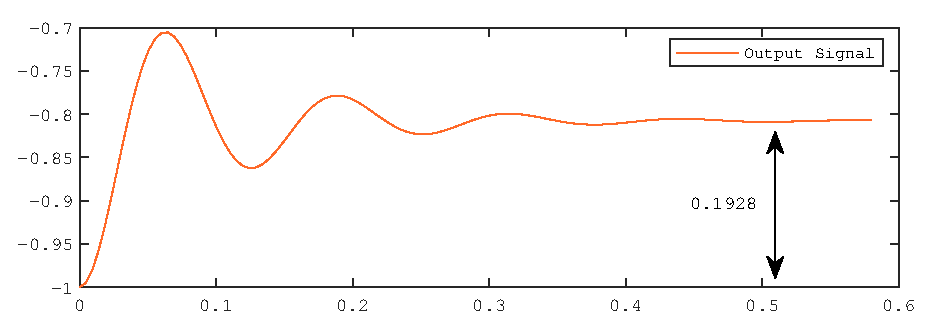
\includegraphics{images/Lab_1_SettlingTime_1.eps}%
  }\hfill
  \subfloat[Zoomed-in view on the settling behaviour of signal.%
  \label{fig:lab1:settling-time:b}]{%
    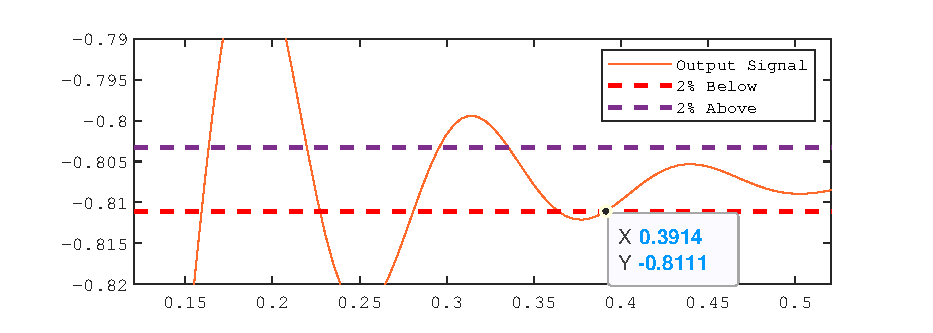
\includegraphics{images/Lab_1_SettlingTime_2.eps}%
  }
  \caption[Step Response for a Linear Plant depicting Settling Time Measurements]{
    The step response of some unknown plant with the \(2\%\)-settling time
    annotated in part (b). Observe how the the signal stays in
    the \(2\%\) region, demarcated by the broken lines,
    after the settling time of \(\SI{391.4}{ms}\) is attained.
  }
  \label{fig:lab1:settling-time}
\end{figure}
%
The settling time is a measure of long-term behaviour.
The notion is best depicted by Figure
\ref{fig:lab1:settling-time}.
In Figure~\ref{fig:lab1:settling-time:a} the ``net'' final value is
measured \emph{from the base to the top} of the signal. Then \(2\%\) of the
settling value is computed to define a cut-off point above and below the final
value, depicted as the broken lines in Figure
\ref{fig:lab1:settling-time:b}. Notice how the signal \emph{stays} in the
settling region after the settling time.
The next characteristic of the step response worthy of measurement is the
time constant.
%
\begin{definition}[]{The Time Constant}
  For a first order plant \(P(s)\) and step input \(U(s) = \frac{1}{s},\)
  the \textbf{time constant} is the time \(\tau > 0\) it takes for
  the output \(y(t)\) to reach \(63\%\) of its final value.
\end{definition}
%
The time constant is a measure of transient, short-term behaviour. Note that,
unlike the settling time, the time constant only has meaning for a
first-order system of the form \(\frac{K}{s + p}.\) You will derive the
relationship as one of your deliverables.
%
\begin{procedure}[label={proc:lab1:p4}]
  In this procedure you will acquire the settling time and time constant
  of your plant \(P(s).\) First, \textbf{ensure} your plant is in open-loop
  configuration.
  \begin{enumerate}[label=(\arabic*)]
    \item{
      \textbf{Open} the signal generator block and \textbf{set} the type
      to be a square wave. Also, \textbf{set} the frequency to a low value,
      such as \(\SI{0.5}{Hz}.\) You will want to see atleast one step in
      the simulation but not too many more than that.
    }
    \item{
      \textbf{Run} the script \texttt{generate\_lab\_1\_plot.m} and inspect
      Figure 1, which depicts the input and output signal.
    }
    \item{
      Using cursors, \textbf{measure} the ``net'' final value by measuring from
      \emph{the base value of the signal to the final value}.
    }
    \item{
      Using the above measurement, \textbf{calculate} the \(63\%\) point
      where the time constant is found and \textbf{calculate} the \(2\%\)
      margins where the settling time is found.
    }
    \item{
      Using cursors, \textbf{measure} the time constant and settling times.
    }
  \end{enumerate}
\end{procedure}
%
\begin{deliverable}[label={lab1:d4}]
  \textbf{Capture the figure} you used to measure the settling time and
  time constant in Procedure~\ref{proc:lab1:p4}. \textbf{Show} your cursors.
\end{deliverable}
%
\begin{procedure}[label={proc:lab1:p5}]
  Repeat Procedure~\ref{proc:lab1:p4} for the closed-loop system described in
  Procedure~\ref{proc:lab1:p3}.
\end{procedure}
%
\begin{deliverable}[label={lab1:d5}]
  \textbf{Capture the figure} you used to measure the settling time and
  time constant in Procedure~\ref{proc:lab1:p5}. \textbf{Show} your cursors.
\end{deliverable}
%

\subsection{On Saturation or Clipping}
In practice, unlike in simulation, the signals we can apply to a system are
limited. This may be an inherent limitation, e.g.
power supply limitations, or a self-imposed safety limitation, e.g.
the angular velocity of an autonomous vehicle. Understanding where these hard
constraints appear in your control system is important, as usually these
constraints have \emph{nonlinear} effects! Ideally, we want to remain in
the region which has linear behaviour.

The only type of constraint you will encounter in these labs is the saturator
constraint. A \textbf{saturator}, or \textbf{clipper} as it is known in
electronics, limits a signal's maximum and minimum value to some preset
constant. In this section, you will attempt to find this limit.
%
\begin{procedure}[label={proc:lab1:p6}]
  \textbf{Put} your system in open-loop. \textbf{Set} the signal generator to
  generate a sinusoid with amplitude \(1\) at a low frequency.
  \textbf{Set} the gain \(K_p\) to \(1\) and \textbf{simulate}.
  \textbf{Increase} the gain \(K_p\) and \textbf{simulate} until you can
  observe the effects of saturation.
\end{procedure}
%
\begin{deliverable}[label={lab1:d6}]
  \textbf{Capture} the figure depicting the effects of saturation.
  \textbf{Record} the value of \(K_p\) where you had clipping occur.
\end{deliverable}

\section{Report Deliverable}
Good job! You made it through Lab 1. You are required to submit a report
that verifies you completed Lab 1 and that you understand the procedures you
performed. In addition to including
\begin{itemize}
  \item{Deliverable~\ref{lab1:d1},}
  \item{Deliverable~\ref{lab1:d2},}
  \item{Deliverable~\ref{lab1:d3},}
  \item{Deliverable~\ref{lab1:d4},}
  \item{Deliverable~\ref{lab1:d5} and}
  \item{Deliverable~\ref{lab1:d6}}
\end{itemize}
in your report,
you are required to answer the questions of the following deliverable.
Make sure to leverage your other deliverables in your answers!
\begin{deliverable}[label={lab1:report}]
  \begin{enumerate}[label={(\arabic*)}]
    \item{
      \textbf{Derive} a formula for the DC gain of \(P(s)\) in terms of
      \(a, b, T.\)
      \emph{Hint: Recall that the DC gain for a stable system \(G(s)\)
      is just \(G(0).\)}
      \label{lab1:report:q1}
    }
    \item{
      You know that your plant takes the form
      \[
        P(s) = \frac{b T}{s + a T},
      \]
      for \(a, b > 0\) and \(T \in \{10, 100\}.\) \textbf{Derive} a
      formula for the bandwidth of \(P(s)\) in terms of \(a, b, T.\)
      \emph{Hint: Remember that the bandwidth frequency \(\omega\) solves
      the equation}
      \[
        \frac{\left\|P(j \omega)\right\|}{\left\|P(0)\right\|}
        =
        \frac{1}{\sqrt{2}}.
      \]
      \emph{Can you explain why? Solve the expression for \(\omega.\) As
      an additional hint, you should get a polynomial in \(\omega^2\) which
      you can solve.}
      \label{lab1:report:q2}
    }
    \item{
      Using the formulas you derived in~\ref{lab1:report:q1} and
      \ref{lab1:report:q2} and the estimates of your bandwidth and DC gain
      in Procedures~\ref{proc:lab1:p1} and~\ref{proc:lab1:p2},
      \textbf{estimate} \(a, b, T.\) Recall that \(T\) can only take on
      values \(10\) or \(100.\)
      \label{lab1:report:q3}
    }
    \item{
      \textbf{Compare} the estimates of \(a, b, T\) made in
      \ref{lab1:report:q3} to your actual parameters.
      \textbf{Open} the ``\texttt{Lab\_1\_Data.sldd}'' to see your plant
      parameters. If there are discrepencies, explain why.
      \label{lab1:report:q4}
    }
    \item{
      \textbf{Find} a formula for the time constant of \(P(s)\) in terms of
      \(a, b, T.\) \emph{Hint: If you put \(P(s)\) in standard first order
      form, can you see what the time constant is?}
      \label{lab1:report:q5}
    }
    \item{
      \textbf{Find} the formula for the \(2\%\) settling time of \(P(s)\) in terms of \(a, b, T.\)
      \emph{Hint: You know \(P(s),\) the input \(U(s) = \frac{1}{s}\) and that
      the output is}
      \[
        Y(s) = P(s) U(s).
      \]
      \emph{Solve for an explicit expression for \(y(t)\) in the time domain.
      Then find how long it takes to reach \(2\%\) of the DC gain (the steady
      state value for a unit step)}
      \label{lab1:report:q6}
    }
    \item{
      Using the formulas you derived in~\ref{lab1:report:q5} and
      \ref{lab1:report:q6} and the estimates of your settling time and
      time constant in Procedure~\ref{proc:lab1:p4},
      \textbf{estimate} \(a, b, T.\)
      \label{lab1:report:q7}
    }
    \item{
      \textbf{Compare} the estimates of \(a, b, T\) made in
      \ref{lab1:report:q7} to your actual parameters.
      \label{lab1:report:q8}
    }
    \item{
      \textbf{Find} the transfer
      function from the input to the output when the system is in
      closed-loop, treating \(a, b, T, K_p\) as just unknown parameters.
      \emph{Hint: In closed loop you can write \(P(s) = K_p(R(s) - Y(s))\)
      where \(R(s)\) is the input to the loop summing junction. See
      Figure~\ref{fig:lab1:closing-loop}.
      Rewrite in the form \(Y(s) = G(s) R(s)\) where \(G(s)\) is the
      transfer function. Put \(G(s)\) in standard first order form.}
      \label{lab1:report:q9}
    }
    \item{
      \textbf{Discuss} how closing the loop, in Procedure
      \ref{proc:lab1:p3}, affected the bandwidth and DC gain.
      \textbf{Justify} your answer using the transfer function
      found in~\ref{lab1:report:q9}.
      \label{lab1:report:q10}
    }
    \item{
      \textbf{Discuss} how closing the loop, in Procedure
      \ref{proc:lab1:p5}, affected the settling time and time constant.
      \textbf{Justify} your answer using the transfer function
      found in~\ref{lab1:report:q9}.
      \label{lab1:report:q11}
    }
    \item{
      \textbf{Discuss} why we want to know the saturator limits. What would
      happen if we performed control design without verifying our control
      stayed within limits?
      \label{lab1:report:q12}
    }
  \end{enumerate}
\end{deliverable}

\subsection{Grading Scheme}
The grading scheme is shown in Table~\ref{tab:lab1:grading}. The breakdown of
your grade is shown per deliverable except in the case of the lab
questions where it is shown per question.
%
\begin{table}
\centering
\begin{tabular}{c|l|c}
        & Deliverable           & Marks  \\ \hline
        & \ref{lab1:d1}         & 2       \\ \hline
        & \ref{lab1:d2}         & 2       \\ \hline
        & \ref{lab1:d3}         & 2       \\ \hline
        & \ref{lab1:d4}         & 2       \\ \hline
        & \ref{lab1:d5}         & 2       \\ \hline
        & \ref{lab1:d6}         & 2       \\ \hhline{=|=|=}
Lab Subtotal&                       & 12      \\ \hhline{=|=|=}
        & \ref{lab1:report}~\ref{lab1:report:q1}  & 1       \\ \hline
        & \ref{lab1:report}~\ref{lab1:report:q2}  & 1       \\ \hline
        & \ref{lab1:report}~\ref{lab1:report:q3}  & 3       \\ \hline
        & \ref{lab1:report}~\ref{lab1:report:q4}  & 3       \\ \hline
        & \ref{lab1:report}~\ref{lab1:report:q5}  & 1       \\ \hline
        & \ref{lab1:report}~\ref{lab1:report:q6}  & 1       \\ \hline
        & \ref{lab1:report}~\ref{lab1:report:q7}  & 3       \\ \hline
        & \ref{lab1:report}~\ref{lab1:report:q8}  & 3       \\ \hline
        & \ref{lab1:report}~\ref{lab1:report:q9}  & 1       \\ \hline
        & \ref{lab1:report}~\ref{lab1:report:q10} & 5       \\ \hline
        & \ref{lab1:report}~\ref{lab1:report:q11} & 5       \\ \hline
        & \ref{lab1:report}~\ref{lab1:report:q12} & 1       \\ \hhline{=|=|=}
Report Subtotal&  & 28 \\ \hhline{=|=|=}
  Total &                       & 40
\end{tabular}
\caption[Grading Scheme for Lab 1]{Grading scheme for Lab 1.}
\label{tab:lab1:grading}
\end{table}
%
